%versi 2 (8-10-2016) 
\chapter{Pendahuluan}
\label{chap:intro}
   
\section{Latar Belakang}
\label{sec:label}

Aplikasi pratinjau 3 dimensi merupakan sebuah perangkat lunak yang membantu penggunanya untuk meninjau kembali desain dari produk yang ingin dihasilkan secara 3 dimensi, sebelum pengguna tersebut melakukan implementasi pembuatan produk. Kelebihan dari aplikasi ini adalah pengguna dapat melakukan peninjauan dari berbagai sudut pandang untuk memaksimalkan hasil dari implementasi pembuatan produk. Aplikasi pratinjau tiga dimensi juga memungkinkan pengguna untuk merubah desain dari produk, hal ini bertujuan agar dapat membantu pengguna memutuskan desain produk yang paling sesuai. Pada dasarnya aplikasi pratinjau tiga dimensi bertujuan untuk membantu pengguna agar terhindar dari hasil pembuatan produk yang tidak sesuai dengan ekspektasi pengguna.

Penggunaan teknologi {\it web} pada aplikasi 3 dimensi dapat memudahkan pengguna untuk melakukan akses aplikasi tanpa harus melakukan instalasi aplikasi namun hanya menggunakan {\it  browser}. Kemudian aplikasi berbasis web juga ramah untuk berbagai lingkungan sistem operasi seperti Windows, Linux, dan Mac OS sehingga tidak membatasi cakupan penggunanya.

Pada skripsi ini, akan dibuat aplikasi pratinjau 3 dimensi berbasis web yang dapat memungkinkan pengguna untuk melakukan kustomisasi ruang belajar mengajar pada lingkungan perkuliahan. Melalui perangkat lunak ini, pengguna diharapkan dapat memiliki gambaran 3 dimensi mengenai ruangan belajar mengajar dengan komposisi warna dinding dan tekstur lantai yang tepat. Perangkat lunak akan dibuat dengan memanfaatkan WebGL dan pustaka Three.js. WebGL merupakan sebuah lintas platform, standar web bebas royalti untuk {\it Application Programming Interface} (API) grafis 3 dimensi level rendah yang berdasar dari OpenGL ES, terbuka untuk ECMAScript melalui elemen {\it canvas} HTML5. Sementara itu pustaka Three.js bertujuan membuat pustaka 3 dimensi yang mudah dan ringan untuk digunakan. Kemudian sebagai studi kasus, ruangan belajar mengajar yang akan digunakan untuk melakukan simulasi aplikasi pratinjau tiga dimensi berbasis {\it web} adalah salah satu ruangan perkuliahan di Fakultas Teknologi Informasi dan Sains. Ruangan tersebut dilengkapi dengan peralatan multimedia yang dapat menunjang pengajaran berbasis Teknologi Informasi seperti komputer, proyektor, serta koneksi internet yang dapat menunjang perkuliahan berbasis E-learning. Selain itu untuk menjamin kenyamanan selama perkuliahan, semua ruang kuliah dilengkapi pendingin udara.

\begin{figure}
	\centering
	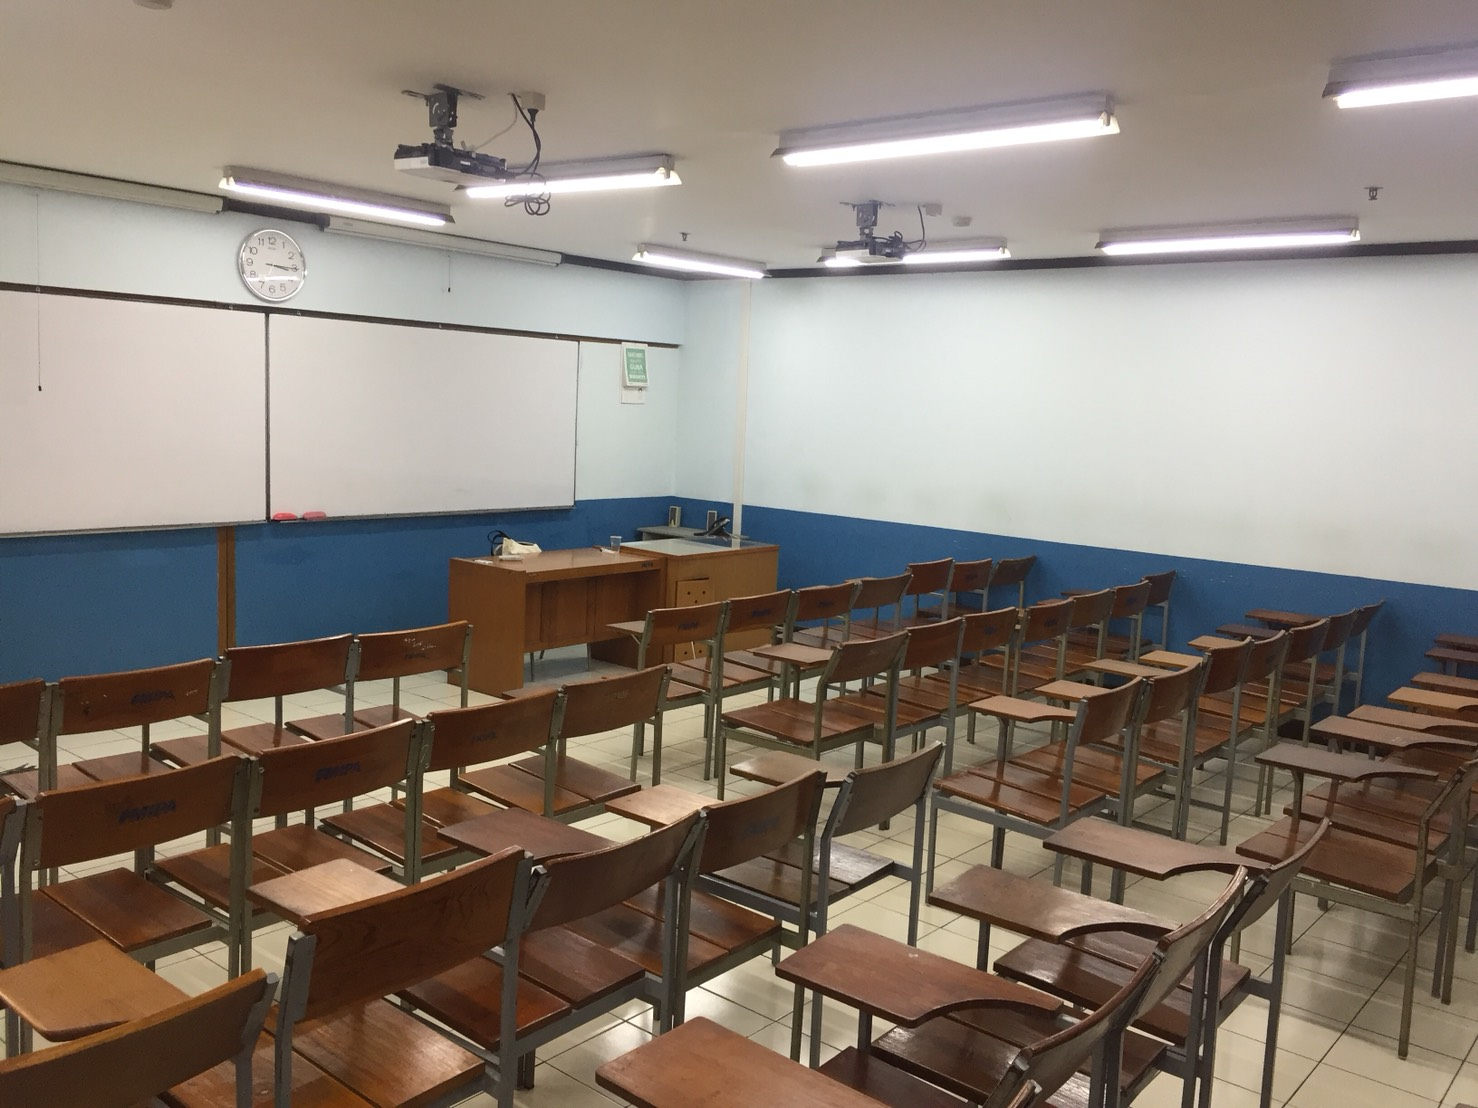
\includegraphics[scale=0.28]{classbyn1}
	\caption{ruangan perkuliahan di Fakultas Teknologi Informasi dan Sains (1)}
	\vspace{8mm}
	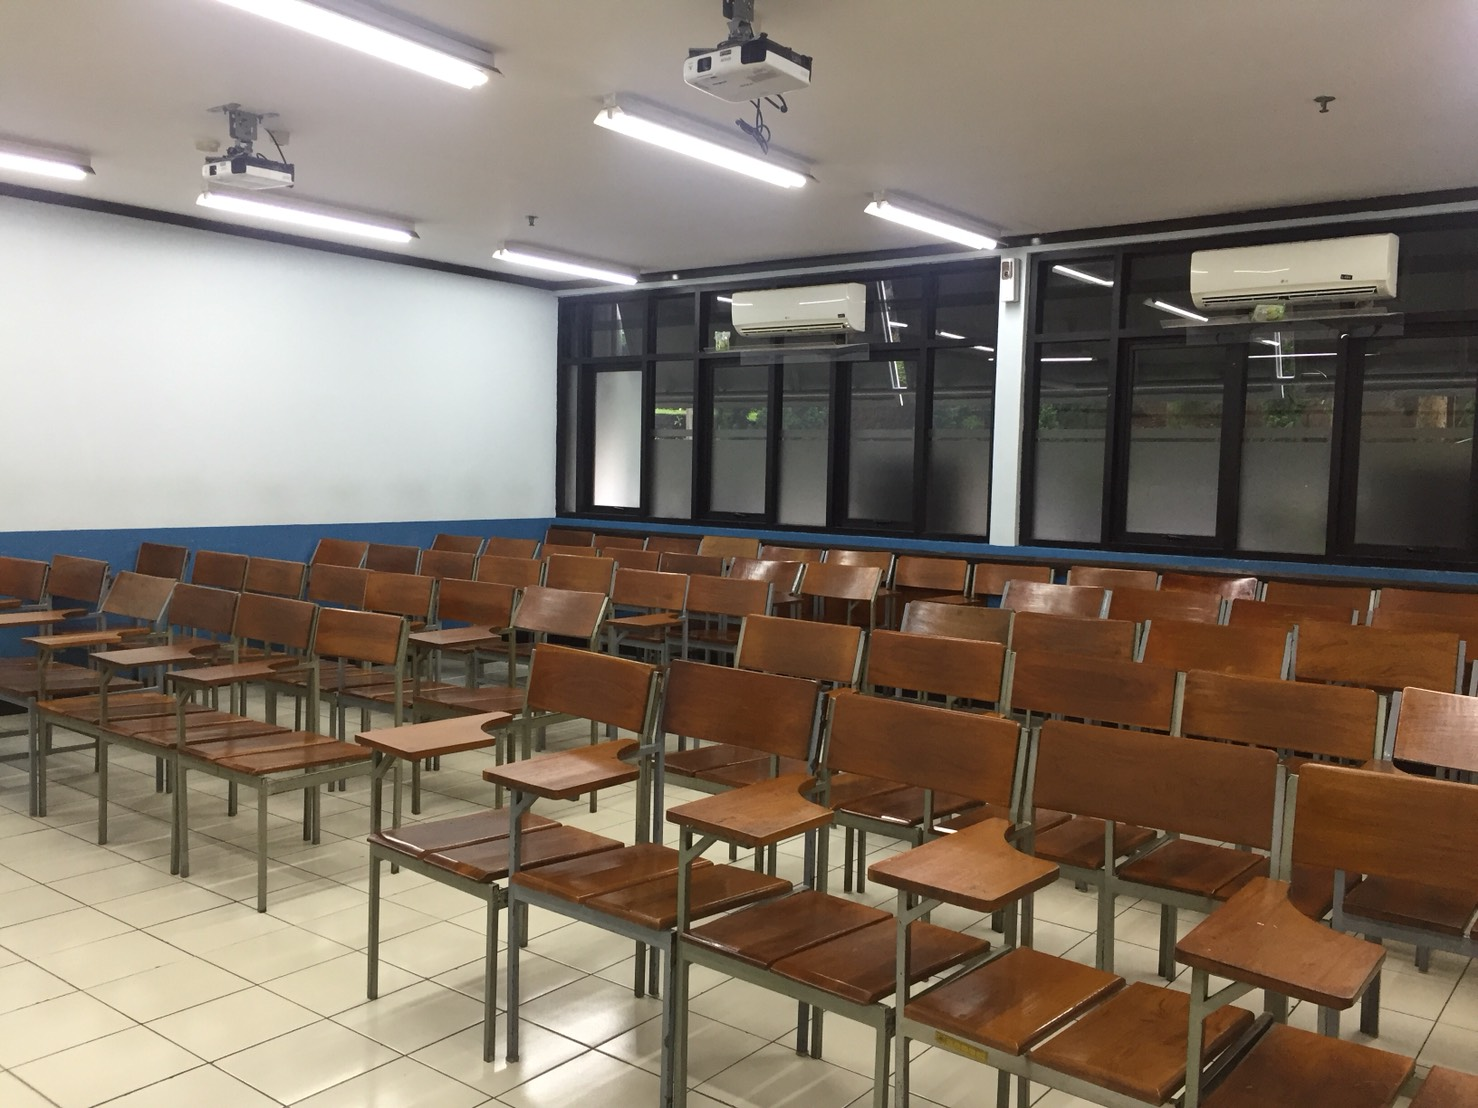
\includegraphics[scale=0.28]{classbyn3}
	\caption{ruangan perkuliahan di Fakultas Teknologi Informasi dan Sains (2)}
\end{figure}

\section{Rumusan Masalah}
\label{sec:rumusan}
Berikut ini masalah-masalah yang dibahas dalam skripsi ini:
\begin{itemize}
    \item Bagaimana ruangan kelas dan objek pendukung lainnya dapat direpsentasikan dalam WebGL?
    \item Bagaimana membuat tampilan responsif pada aplikasi agar terlihat bagus saat dicetak?
\end{itemize}

\section{Tujuan}
\label{sec:tujuan}
Berikut ini tujuan-tujuan yang ingin dicapai dalam penilitian ini:
\begin{itemize}
    \item Membangun aplikasi yang dapat merepresentasikan ruangan dalam WebGL.
    \item Membangun tampilan aplikasi yang responsif sehingga terlihat bagus saat dicetak.
\end{itemize}

\section{Batasan Masalah}
\label{sec:batasan}
Terdapat beberapa batasan masalah dalam penilitian ini, yaitu:
\begin{enumerate}
    \item Pengguna hanya dapat melakukan kustomisasi pada tekstur lantai, warna cat dinding bagian atas, dan warna cat dinding bagian bawah dari ruangan kelas.
    \item Pengguna hanya dapat mengganti tekstur lantai, warna cat dinding bagian atas, dan warna cat dinding bagian bawah dengan 8 variasi.
    \item Ruangan hanya dalam bentuk persegi atau persegi panjang.
\end{enumerate}
\section{Metodologi}
\label{sec:metlit}
Metodologi yang digunakan untuk menyusun penelitian ini adalah sebagai berikut:
\begin{enumerate}
    \item Mempelajari standar WebGL sebagai \textit{Application Programming Interface} untuk menampilkan grafis 3 dimensi pada \textit{web browser}.
    \item Mempelajari penggunaan Three.js sebagai \textit{library} dari WebGL.
    \item Memodelkan ruangan belajar mengajar secara 3 dimensi.
    \item Melakukan analisis terhadap situs web yang akan dibangun.
    \item Merancang tampilan situs web yang akan dibangun.
    \item Mengimplementasikan situs web.
    \item Melakukan pengujian terhadap situs web yang telah dibangun.
    \item Menulis dokumen skripsi.
\end{enumerate}

\section{Sistematika Pembahasan}
\label{sec:sispem}
Pembahasan dalam buku skripsi ini dilakukan secara sistematis sebagai berikut:
\begin{itemize}
    \item Bab 1 Pendahuluan
    
    Berisi latar belakang, rumusan masalah, tujuan, batasan masalah, metodologi penilitian, dan sistematika pembahasan.
    
    \item Bab 2 Landasan Teori
    
    Berisi teori-teori dasar mengenai WebGL dan Three.js \textit{library}.
    
    \item Bab 3 Analisis
    
    Berisi analisis masalah dan solusi, studi kasus, perancangan perangkat lunak, diagram aktivitas, \textit{use case} diagram, dan diagram paket.
    
    \item Bab 4 Perancangan
    
    Berisi perancangan antarmuka dan diagram kelas.
    
    \item Bab 5 Implementasi
    
    Berisi implementasi antarmuka perangkat lunak, implementasi menggunakan WebGL dan \textit{library} Three.js, pengujian perangkat lunak yang telah dibangun, dan kesimpulan berdasarkan pengujian.
    
    \item Bab 6 Kesimpulan dan Saran
    
    Berisi kesimpulan berdasarkan pengujian yang telah dilakukan dan saran untuk penelitian berikutnya.
\end{itemize}